
%----------------------------------------------------------------------------------------------------------------
\begin{frame}{Results}
\begin{tabular}[h]{@{} p{0.38\linewidth} p{0.38\linewidth}@{}}

\raisebox{0.08\height}{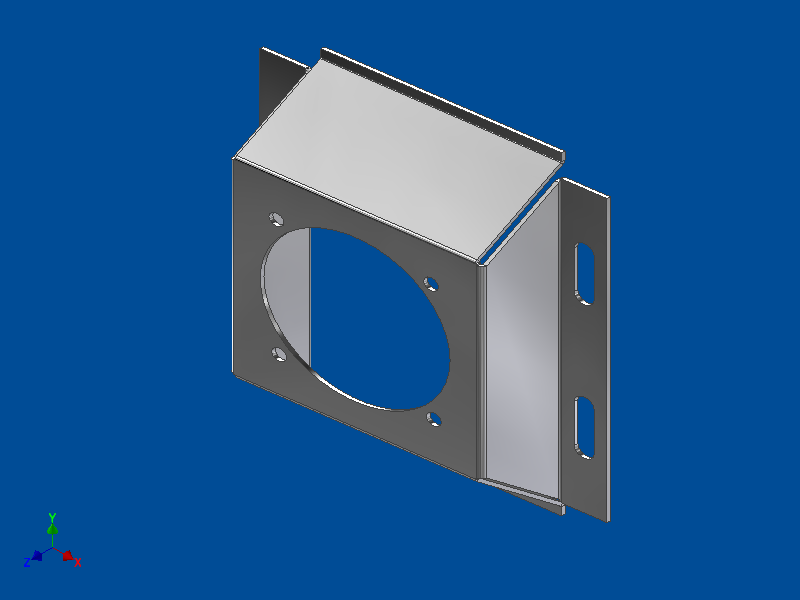
\includegraphics[width=0.75\linewidth]{..//Common/images/SheetMetal_Remnant_Before.png}} &
\raisebox{0.08\height}{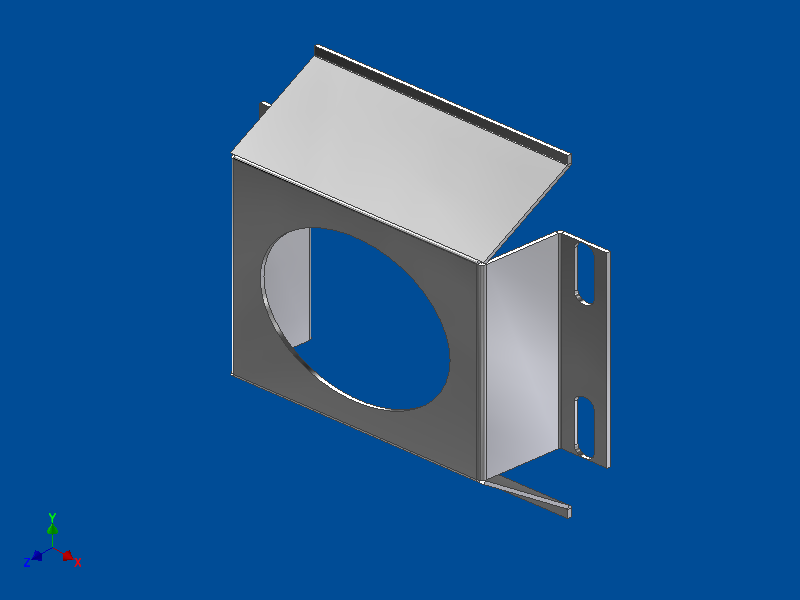
\includegraphics[width=0.75\linewidth]{..//Common/images/SheetMetal_Remnant_After.png}} \\

\raisebox{0.08\height}{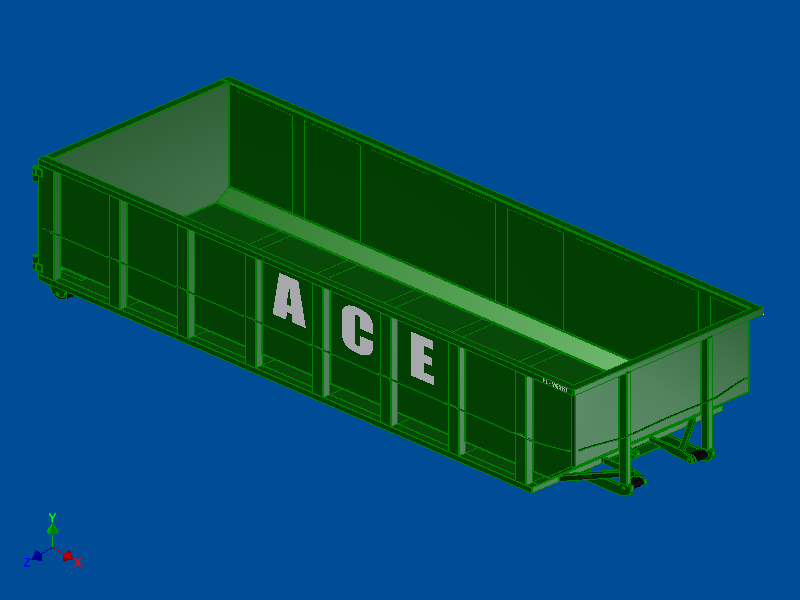
\includegraphics[width=0.75\linewidth]{..//Common/images/SheetMetal_Complex_Dumpster_Remnant_Before.png}} &
\raisebox{0.08\height}{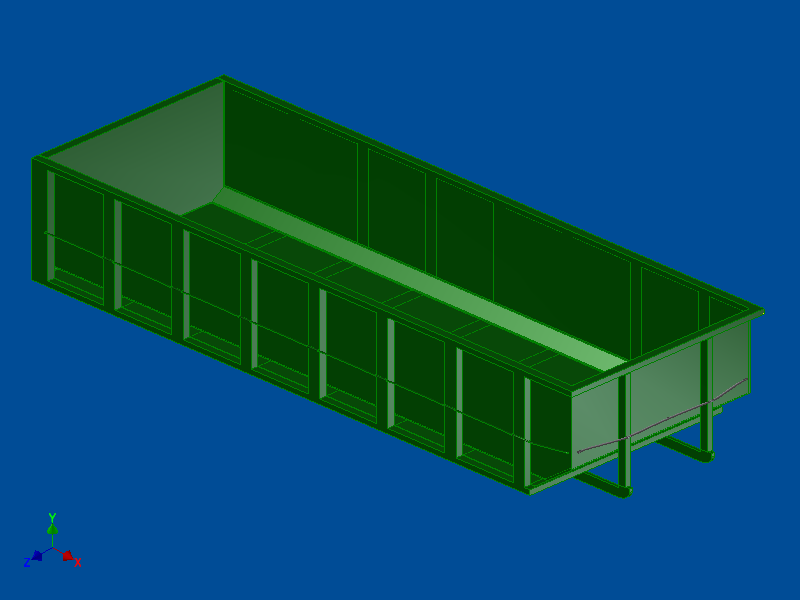
\includegraphics[width=0.75\linewidth]{..//Common/images/SheetMetal_Complex_Dumpster_Remnant_After.png}}\\

\raisebox{0.08\height}{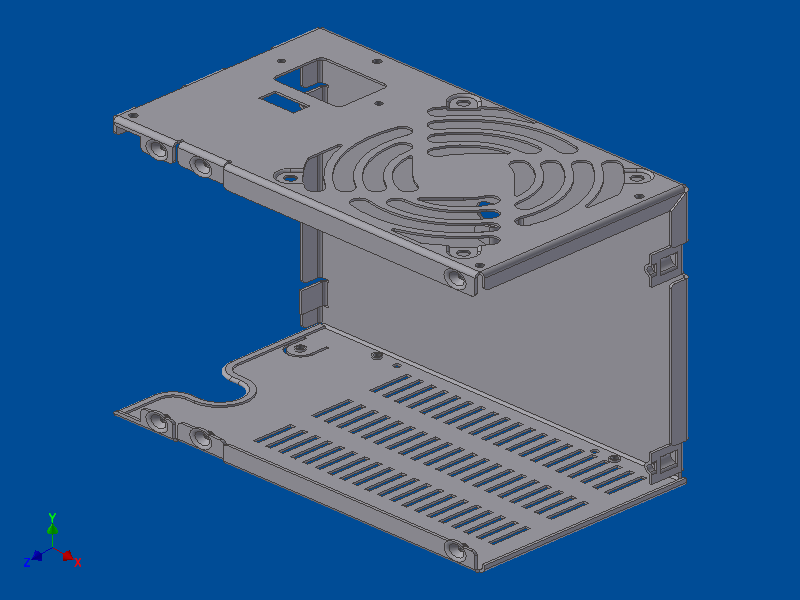
\includegraphics[width=0.75\linewidth]{..//Common/images/SheetMetal_Complex_FoldedPowerSupplyBoxCover_Remnant_Before.png}} &
\raisebox{0.08\height}{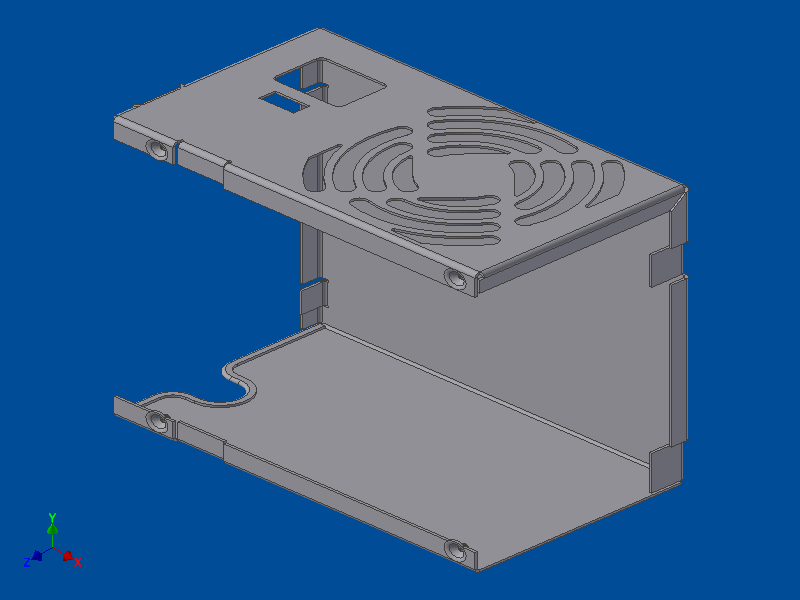
\includegraphics[width=0.75\linewidth]{..//Common/images/SheetMetal_Complex_FoldedPowerSupplyBoxCover_Remnant_After.png}} \\
\end{tabular}
\end{frame}
%------------------------------------------------------------------------------------
\begin{frame}{Comparison}
\begin{tabular}[h]{@{} p{0.16\linewidth}| p{0.16\linewidth} | p{0.16\linewidth}| p{0.16\linewidth} | p{0.16\linewidth}@{}}

& \textbf{Hamdi} &	\textbf{Sungchan} &	\textbf{Lee} &	\textbf{Smarf}\\
\midrule
\textbf{Input} &	Features	& Brep	& Features	& Features\\
\midrule
\textbf{Method}& Find Feature size, compare with threshold, suppress.&
&

Features converted to volumetric +ve, -ve. Reordered.	&
Specific rules for SM features. Remnant face logic\\
\midrule
\textbf{+ve -ve} & For FEM as BC/ Load path features suppressed &
Concave-edge-filling creates odd shapes. &
Update capability is LOST forever. &
Advantages of Feature and Brep approaches\\	
\bottomrule
\end{tabular}
\end{frame}
%------------------------------------------------------------------------------------